\newpage
\subsection{Rademacher Complexity of ramp loss for neural networks}
\subsubsection{Problem Statement}
\label{sec:rad_complexity_of_ramp_loss_nn}
\textbf{Problem} : Given a tuple $\begin{pmatrix}\M{1} & \dots & \M{L}\end{pmatrix}$ of $L\ge 1$ reference matrices (that represents initial weights in a neural network). Let $\mathcal{A}$ be the class of tuples of $L$ weight matrices defined as followed:
\begin{align*}
    \mathcal{A} = \bigCurl{
        \begin{pmatrix}
            \A{1} & \dots & \A{L}
        \end{pmatrix} : \|\A{i}\|_\sigma \le s_i, \|(\A{i} - \M{i})^T\|_{2, 1}\le a_i, \|\A{L} - \M{L}\|_F \le a_*
    }
\end{align*}

\noindent Where $\|.\|_\sigma$ denotes the spectral norm and $\|.\|_{p, q}$ denotes the matrix $(p, q)$ norm defined as $\|A\|_{p, q} = \bigRound{\sum_j\bigRound{\sum_{i}|A_{ij}|^p}^{q/p}}^{1/q}$. Define the following class of neural networks:
\begin{align*}
    \F_\mathcal{A} = \biggCurl{
        x\mapsto \A{L} \biggRound{
            \bigO_{k=1}^{L-1} \sigma_k \circ \A{k}
        }(x) : \sigma_k \text{ is } \rho_k\text{-Lipchitz}, \begin{pmatrix}
            \A{1} & \dots & \A{L}
        \end{pmatrix} \in \mathcal{A}
    }
\end{align*}

\noindent Derive the bound for the Rademacher Complexity of the loss function class:
\begin{align*}
    \mathcal{L}_r = \biggCurl{
        (x, y) \mapsto l_r\bigRound{
            F_\vecbf{A}(x)_y - \max_{k\ne y}F_\vecbf{A}(x)_k
        } \Bigg| F_\vecbf{A} \in \F_\mathcal{A}
    }
\end{align*}

\noindent Where $l_r$ is the ramp loss function with margin $r\in(0,1)$.

\subsubsection{Neural networks covering bounds with general norm}
\begin{theorem}{Neural networks covering bound with general norm}{nn_cover_bound_with_general_norm}
    Let $L \ge 1$ be a natural number and $\epsilon_1, \dots, \epsilon_L > 0$ be given as covering number granularities. Given the following:
    \begin{itemize}
        \item A sequence of vector spaces $\mathcal{V}_0, \dots, \mathcal{V}_L$ endowed with norms $|.|_0, \dots, |.|_L$.
        \item A sequence of vector spaces $\mathcal{W}_1, \dots, \mathcal{W}_L$ endowed with norms $\|.\|_1, \dots, \|.\|_L$.
        \item A sequence of real positive numbers $c_1, \dots, c_L$ and linear operators $\A{i} : \mathcal{V}_i \to \mathcal{W}_{i+1}$ associated with the operator norm:
        \begin{align*}
            \|\A{i}\|_{op} = \sup_{|Z|_i \le 1} \|A_iZ\|_{i+1} \le c_i, \ \forall i \in \{1, \dots, L\}
        \end{align*}

        \item A sequence of real positive numbers $\rho_1, \dots, \rho_L$ and activation functions $\sigma_i:\mathcal{W}_i \to \mathcal{V}_i$ such that $\sigma_i$ are $\rho_i$-Lipchitz:
        \begin{align*}
            |\sigma_i(z_1) - \sigma_i(z_2)|_i \le \rho_i\|z_1 - z_2\|_i
        \end{align*}

        \item Let $\mathcal{A}\subseteq \mathcal{B}_1\times\dots\times\mathcal{B}_L$ be a class of tuples of matrices $(\A{1}, \dots, \A{L})$ such that each $\A{i} \in \mathcal{B}_i$ satisfies $\|\A{i}\|_{op} \le c_i$.

        \item Define the class of neural networks $\F_\mathcal{A}$ as followed:
        \begin{align*}
            \F_\mathcal{A} = \biggCurl{
                x\mapsto \A{L}\biggRound{
                    \bigO_{k=1}^{L-1}\sigma_k \circ \A{k}
                }(x) : (\A{1}, \dots, \A{L}) \in \mathcal{A}
            }
        \end{align*}
        
        \item Let $\tau$ be the aggregated granularity defined as:
        \begin{align*}
            \tau = \sum_{j=1}^L \epsilon_j \rho_j \prod_{l=j+1}^L \rho_lc_l
        \end{align*}
    \end{itemize}
\end{theorem}

\begin{proof*}[Theorem \ref{thm:nn_cover_bound_with_general_norm}]
    \begin{figure}[!ht]
        \centering
        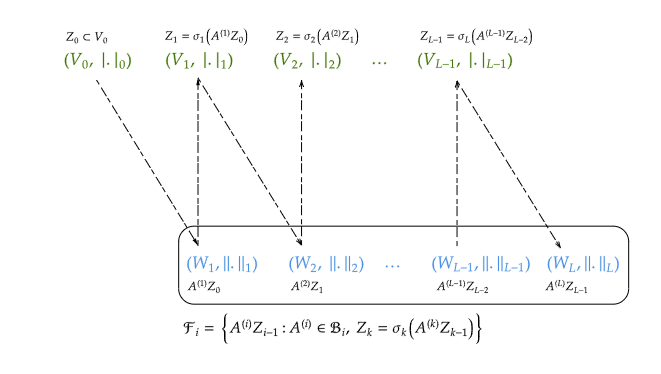
\includegraphics[width=\textwidth]{figures/neural-network.png}
        \caption{Illustration of a feedforward pass of a deep neural network with weight matrices $\vecbf{A}=\Big( \A{1}, \dots, \A{L} \Big)$}
        \label{fig:neural-network-illustration}
    \end{figure}

    \noindent We will prove the above theorem inductively. Suppose we have a sample dataset $Z_0\subset\mathcal{V}_0$. Construct a minimum $\epsilon_1$-cover for $\F_1 = \bigCurl{\A{1}Z_0 : A_1 \in \mathcal{B}_1}$ called $\mathcal{C}_1$. Hence, for all $\A{1}\in\mathcal{B}_i$, there exists $\overline{\A{1}}\in\mathcal{C}_1$ such that:

    \begin{align*}
        \Big\|\A{1}Z_0 - \overline{\A{1}}Z_0\Big\|_1 \le \epsilon_1
    \end{align*} 
    
    
    \noindent For $i\ge 2$, define the class:
    \begin{align*}
        \F_i = \biggCurl{
            \A{i}Z_{i-1} : \A{i} \in \mathcal{B}_i, Z_{i-1} = \sigma_{i-1}\bigRound{\A{i-1}Z_{i-2}}
        }
    \end{align*}


    \noindent Suppose we have a minimum $\epsilon_{i-1}$-cover $\mathcal{C}_{i-1}$ of $\F_{i-1}$. Meaning, for all $\A{i-1}\in\mathcal{B}_{i-1}$, there exists $\overline{\A{i-1}}\in\mathcal{C}_{i-1}$ such that:
    \begin{align*}
        \Big\|\A{i-1}Z_{i-2} - \overline{\A{i-1}}Z_{i-2}\Big\|_{i-1} \le \epsilon_{i-1}
    \end{align*}

    \noindent For each element 
\end{proof*}


\subsubsection{Solution to \ref{sec:rad_complexity_of_ramp_loss_nn}}

